\documentclass[11pt,a4paper]{report}
\usepackage[utf8]{inputenc}
\usepackage[english]{babel}
\usepackage{amsmath}
\usepackage{graphicx}
\usepackage{hyperref}
\usepackage{geometry}
\usepackage{listings}
\usepackage{xcolor}
\usepackage{longtable}
\usepackage{booktabs}
\usepackage{float}
\usepackage{caption}

\geometry{
    a4paper,
    total={170mm,257mm},
    left=25mm,
    right=20mm,
    top=25mm,
    bottom=25mm,
}

\definecolor{codegreen}{rgb}{0,0.6,0}
\definecolor{codegray}{rgb}{0.5,0.5,0.5}
\definecolor{codepurple}{rgb}{0.58,0,0.82}
\definecolor{backcolour}{rgb}{0.95,0.95,0.92}

\lstdefinestyle{mystyle}{
    backgroundcolor=\color{backcolour},   
    commentstyle=\color{codegreen},
    keywordstyle=\color{blue},
    numberstyle=\tiny\color{codegray},
    stringstyle=\color{codepurple},
    basicstyle=\ttfamily\footnotesize,
    breakatwhitespace=false,         
    breaklines=true,                 
    captionpos=b,                    
    keepspaces=true,                 
    numbers=left,                    
    numbersep=5pt,                  
    showspaces=false,                
    showstringspaces=false,
    showtabs=false,                  
    tabsize=4
}
\lstset{style=mystyle, language=Matlab}

\title{\textbf{Industrial Digital Twin}\\ \Large Comprehensive MATLAB Framework Documentation}
\author{Personal Project Documentation}
\date{\today}

\begin{document}

\maketitle

\begin{abstract}
This document serves as the comprehensive, detailed documentation for a custom-built Industrial Digital Twin framework developed in MATLAB. It covers every class, script, mathematical model, and test suite implemented throughout the project lifecycle. The framework employs Object-Oriented Programming (OOP) to rigorously simulate physical processes, electrical systems, and instrumentation layers, while providing SCADA integration capabilities via a native tag-based historian architecture.
\end{abstract}

\tableofcontents
\newpage

\chapter{Introduction \& Architectural Philosophy}

\section{Project Purpose}
The goal of this project is to provide a robust simulation environment capable of acting as a true ``Digital Twin'' for an industrial plant. Traditional MATLAB scripts often mix physical calculations with control logic and data logging, creating monolithic, hard-to-maintain codebases. This framework adopts strict Object-Oriented Programming (OOP) principles to isolate physical processes, sensor measurement errors, and SCADA data aggregation.

\section{Core Architectural Principles}
\begin{enumerate}
    \item \textbf{Reference Semantics (\texttt{handle} classes):} Every component in the plant is passed by reference. This ensures that when a pump reads from a tank, they are interacting with the exact same memory instance, guaranteeing mass and energy conservation across the simulated plant.
    \item \textbf{Physical Truth vs. Measured Output:} The internal \texttt{State} of a device represents perfect physics. The \texttt{Outputs} represent what a PLC would see. This separation allows the injection of realistic sensor noise without breaking the laws of thermodynamics.
    \item \textbf{Standardized Tag Output:} Every piece of equipment implements a \texttt{getTags()} method, outputting a standard industrial tag format (Name, Value, Unit, Quality, Timestamp) ready for OPC UA or SQL Historians.
\end{enumerate}

\chapter{Core Framework Library}
Located in \texttt{library/core/}, these classes form the backbone of the framework.

\section{\texttt{IndustrialObject.m}}
An abstract base class inheriting directly from MATLAB's \texttt{handle}.
\begin{itemize}
    \item \textbf{Properties:} \texttt{ID} (string identifier), \texttt{Type}, \texttt{Description}.
    \item \textbf{Methods:} Enforces the implementation of \texttt{getTags()}, \texttt{update(dt)}, and \texttt{reset()}.
\end{itemize}

\section{\texttt{Equipment.m}}
The workhorse abstract class inheriting from \texttt{IndustrialObject}. All process and electrical units inherit from this.
\begin{itemize}
    \item \textbf{Standardized Structs:} \texttt{Parameters} (static config), \texttt{State} (dynamic internal variables), \texttt{Inputs} (values driven by external components), \texttt{Outputs} (values visible to external components), \texttt{Faults} (boolean flags).
    \item \textbf{Fault Management:} Provides \texttt{injectFault(name)} and \texttt{clearFault(name)} which interact with child classes to physically alter simulation behavior.
    \item \textbf{Status Tracking:} Tracks whether the equipment is "OK", "FAULTED", or "RUNNING".
\end{itemize}

\chapter{Process Equipment Library}
Located in \texttt{library/process/}, these classes model thermodynamic and hydraulic physics.

\section{\texttt{ETank.m} (Cylindrical Tank)}
Simulates fluid accumulation using mass conservation.
\begin{itemize}
    \item \textbf{Physics:} $dV/dt = Q_{in} - Q_{out} - Q_{leak}$. Level is derived as $h = V / (\pi \cdot r^2)$.
    \item \textbf{Faults:} \texttt{Leakage} (introduces a leak flow proportional to the current head/level), \texttt{SensorFailure} (sets the measured output level to \texttt{NaN} while leaving the physical volume intact).
\end{itemize}

\section{\texttt{EPipe.m} (Pipeline)}
Simulates pressure drop using simplified Darcy-Weisbach friction.
\begin{itemize}
    \item \textbf{Physics:} $\Delta P = R_{friction} \cdot Q^2 + \rho \cdot g \cdot \Delta z$.
    \item \textbf{Faults:} \texttt{Blockage} (multiplies friction resistance by 100), \texttt{Leak} (diverts a percentage of incoming flow so it never reaches the output).
\end{itemize}

\section{\texttt{EPump.m} (Centrifugal Pump)}
Models both hydraulic performance and motor inertia.
\begin{itemize}
    \item \textbf{Physics:} Motor speed approaches target via first-order lag ($\tau \cdot dN/dt = N_{target} - N$). The hydraulic head follows affinity laws: $H = H_{max} \cdot (N/N_{rated})^2 - k \cdot Q^2$. Power draw is proportional to the cube of the speed.
    \item \textbf{Faults:} \texttt{BearingFault} (drops efficiency, artificially increasing power consumption), \texttt{MotorFailure} (speed coasts to zero).
\end{itemize}

\section{Valves: \texttt{EValve.m} \& \texttt{EControlValve.m}}
\begin{itemize}
    \item \textbf{\texttt{EValve}:} Simple on/off valve with a configurable stroke time.
    \item \textbf{\texttt{EControlValve}:} Modulating valve accepting a 0-100\% command. Simulates first-order actuator delay and three flow profiles: Linear, Equal-Percentage ($f(x) = R^{x-1}$), and Quick-Opening ($f(x) = \sqrt{x}$).
    \item \textbf{Faults:} \texttt{StuckOpen}, \texttt{StuckClosed}, \texttt{Stuck} (freezes at current position), \texttt{ActuatorFailure} (drives to a predefined fail-safe state).
\end{itemize}

\section{Advanced Units: \texttt{EMixer}, \texttt{EHeater}, \texttt{EFilter}}
\begin{itemize}
    \item \textbf{\texttt{EMixer}:} Accepts two inflows with varying concentrations. Assumes perfect mixing and calculates the output concentration dynamically. Fault: \texttt{AgitatorFailure}.
    \item \textbf{\texttt{EHeater}:} Adds thermal energy ($Q$) to a flowing mass ($m$). $dT = Q / (m \cdot C_p)$. Fault: \texttt{ElementFailure}.
    \item \textbf{\texttt{EFilter}:} Tracks particulate accumulation over time, causing an exponential increase in pressure drop. Fault: \texttt{Rupture} (pressure drop collapses).
\end{itemize}

\chapter{Electrical \& Actuation Library}
Located in \texttt{library/electrical/}.

\section{\texttt{EMotor.m} \& \texttt{EVFD.m}}
\begin{itemize}
    \item \textbf{\texttt{EMotor}:} An independent motor model. Tracks spin-up time constants and cubic power laws. Faults: \texttt{Overheat}, \texttt{Tripped}.
    \item \textbf{\texttt{EVFD}:} Variable Frequency Drive. Intercepts a 0-100\% setpoint and modulates the attached \texttt{EMotor}'s parameters to simulate variable speed operation. Fault: \texttt{DriveFault}.
\end{itemize}

\section{\texttt{EConveyor.m}}
Simulates material transport. Tracks load ($kg/m$) and speed ($m/s$).
\begin{itemize}
    \item \textbf{Physics:} Transport delay and mass balance across the belt length.
    \item \textbf{Faults:} \texttt{BeltSlip} (speed halves), \texttt{MotorTrip}.
\end{itemize}

\chapter{Instrumentation Layer}
Located in \texttt{library/instrumentation/}.

\section{\texttt{ETransmitter.m} (Base Sensor)}
A wrapper class that reads a specific property from a target \texttt{Equipment} and applies signal degradation.
\begin{itemize}
    \item \textbf{Signal Chain:} 
    $$ Measured = (True \times SpanDrift) + ZeroDrift + \mathcal{N}(0, \sigma^2) $$
    The measured value is then clamped to sensor limits and converted to a 4-20mA electrical signal.
    \item \textbf{NAMUR NE43 Faults:}
    \begin{itemize}
        \item \texttt{SignalLoss}: Wire break. Current drops to 0mA, quality becomes \texttt{BAD\_COMM}.
        \item \texttt{FrozenSignal}: ADC lockup. Signal holds the last value indefinitely (\texttt{UNCERTAIN\_STALE}).
        \item \texttt{CalibrationLoss}: Massive 20\% span error injection.
    \end{itemize}
\end{itemize}

Specialized subclasses (\texttt{ELevelTransmitter}, \texttt{EFlowTransmitter}, \texttt{EPressureTransmitter}) automatically map to specific engineering units and target properties to reduce boilerplate code during instantiation.

\chapter{SCADA \& System Architecture}
Located in \texttt{library/historian/} and \texttt{library/system/}.

\section{\texttt{ETagDatabase.m} (Plant Server)}
Acts as an OPC UA / SCADA server. All equipment must be registered here. The \texttt{scanAll()} method loops through all devices, executes their \texttt{getTags()} methods, and vertically concatenates the results into a \texttt{MasterTagTable}. It maintains a \texttt{containers.Map} for $O(1)$ fast tag lookups.

\section{\texttt{EHistorian.m} (Time-Series Logger)}
Binds to the \texttt{ETagDatabase} and records tag histories.
\begin{itemize}
    \item \textbf{Memory Management:} To prevent MATLAB memory fragmentation during long loops, it utilizes pre-allocated arrays (\texttt{BufferSize}). When the buffer is full, it dynamically doubles in size.
    \item \textbf{Data Retrieval:} \texttt{getHistory("TAG")} slices the active data and returns a native MATLAB \texttt{timetable}, ready for plotting or Machine Learning.
\end{itemize}

\section{\texttt{EFactory.m} \& \texttt{ESimulationEngine.m}}
\begin{itemize}
    \item \textbf{\texttt{EConnection}:} Physically maps the output property of a Source to the input property of a Target, routing flow data automatically.
    \item \textbf{\texttt{EFactory}:} A container holding all Equipment, Connections, Database, and Historian. Its \texttt{update(dt)} method enforces the order of execution: Connections $\rightarrow$ Equipment Physics $\rightarrow$ Database Scan $\rightarrow$ Historian Log.
    \item \textbf{\texttt{ESimulationEngine}:} The execution loop manager that runs the factory for a designated time duration given a discrete time step $\Delta t$.
\end{itemize}

\chapter{Testing and Validation}
The framework was developed using Test-Driven Development (TDD) via the \texttt{matlab.unittest} framework.

\section{Test Coverage}
A total of \textbf{92 automated tests} were written across multiple suites:
\begin{itemize}
    \item \textbf{\texttt{ETankTest.m} (15 tests):} Validates volume conservation, overflow limits, alarms (LL/L/H/HH), leakage dynamics, and fault resets.
    \item \textbf{\texttt{EPumpTest.m}, \texttt{EPipeTest.m}, \texttt{EValveTest.m}:} Verifies Darcy-Weisbach curves, affinity laws, and valve transition times.
    \item \textbf{\texttt{ETransmitterTest.m} (7 tests):} Tests Gaussian noise std-dev validation, signal limits, and NAMUR fault states.
    \item \textbf{\texttt{ETagDatabaseTest.m} \& \texttt{EHistorianTest.m}:} Validates that tag arrays grow correctly, and timetables retain exact values mapped to timestamps.
\end{itemize}
\textbf{Final Result:} 92/92 tests passing with zero failures.

\chapter{Examples \& Use Cases}
Five main examples reside in the \texttt{examples/} directory.

\section{\texttt{TankExample.m}}
This script focuses purely on the hydraulics of static storage. It runs a single tank through a sequence of filling and draining cycles to validate mass conservation and verifies the triggering of Level (L/LL/H/HH) alarms.

\begin{figure}[H]
    \centering
    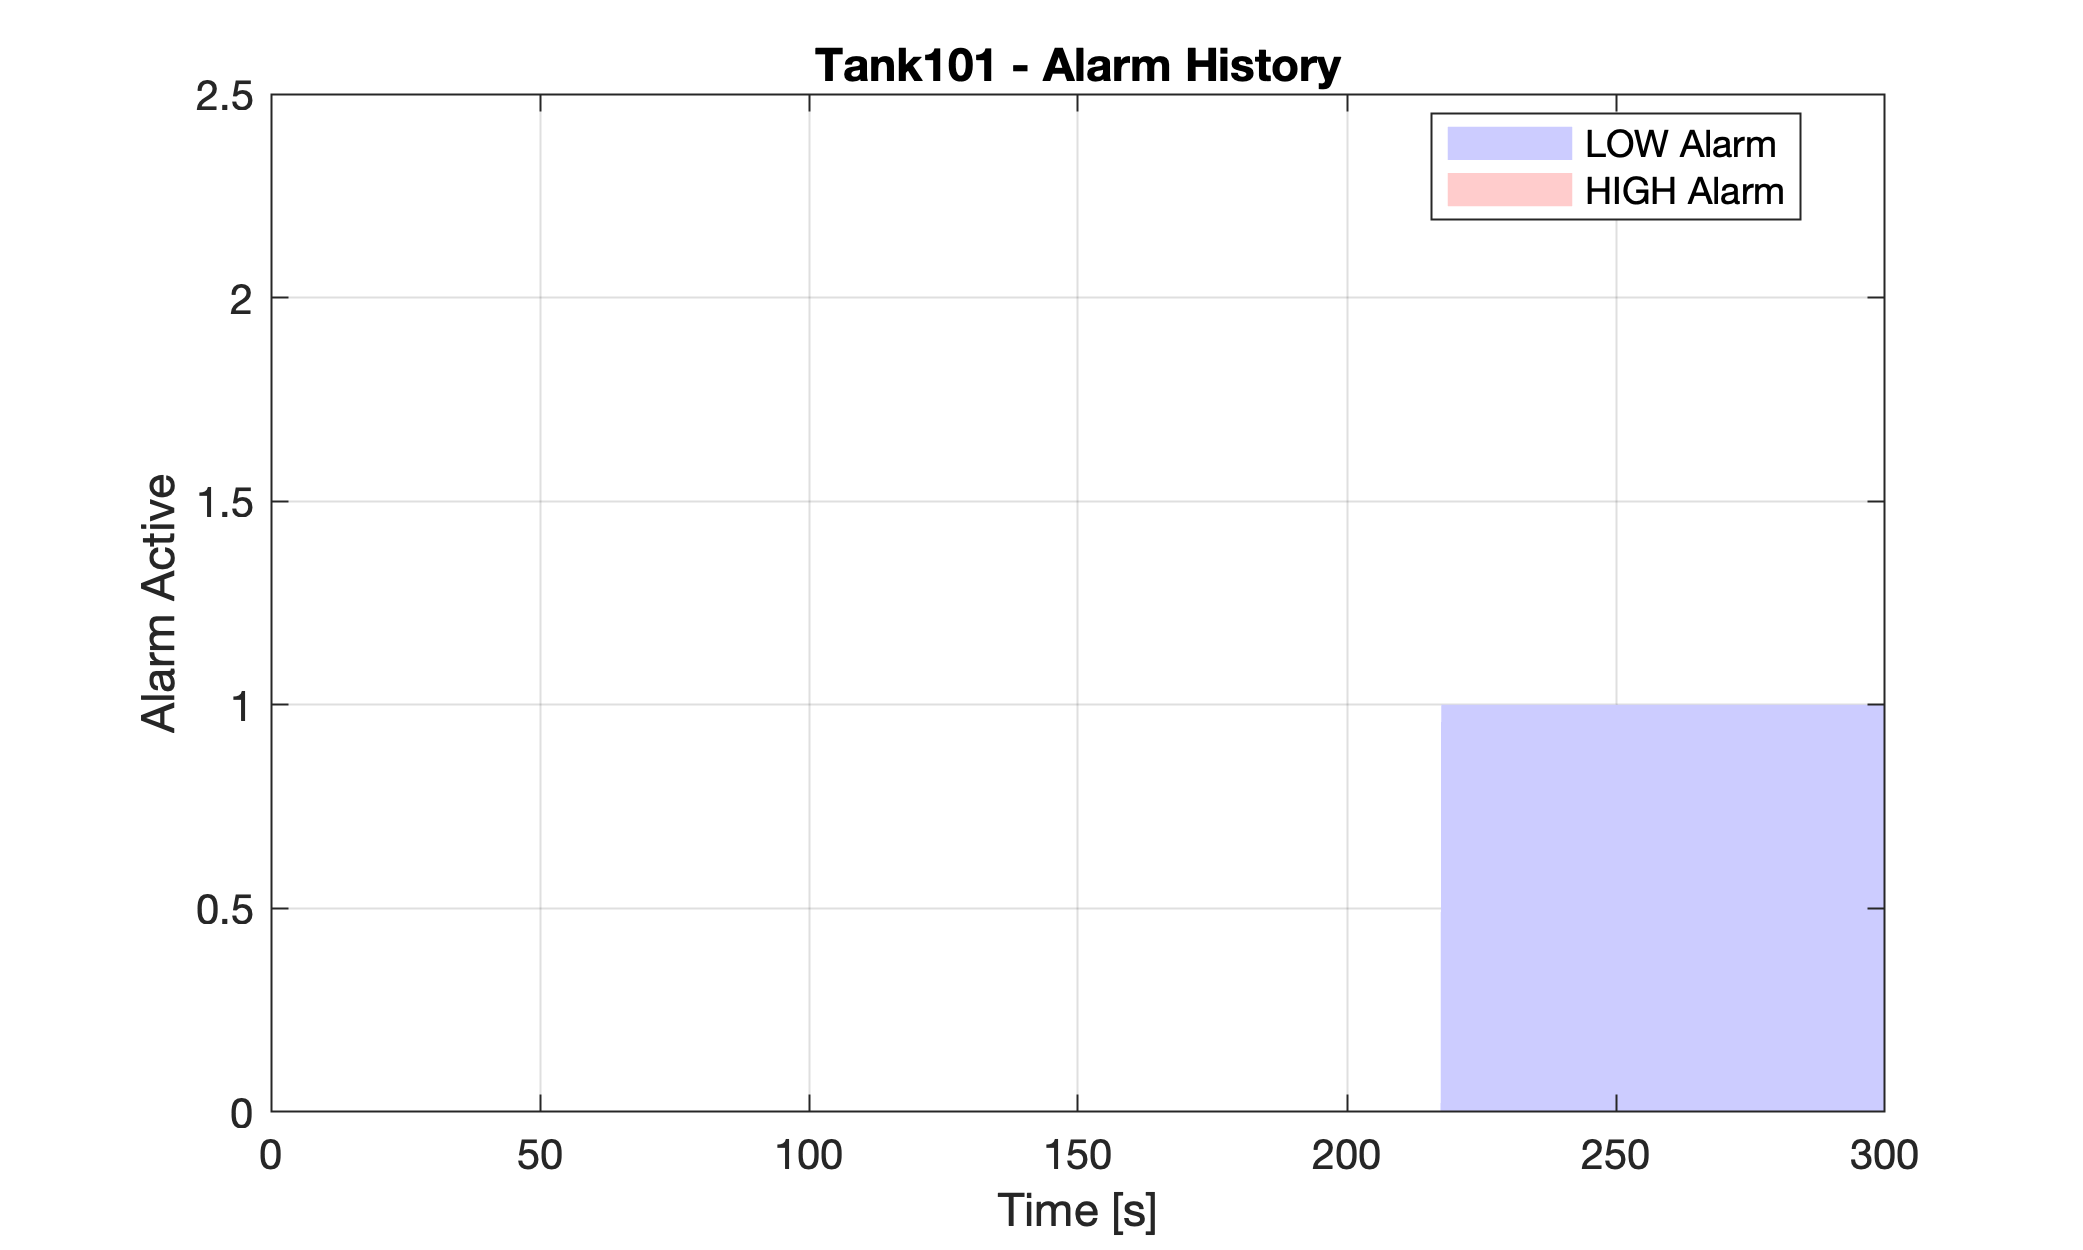
\includegraphics[width=0.9\textwidth]{images/tank_example.png}
    \caption{Tank example showcasing fluid levels, faults, and alarm thresholds.}
    \label{fig:tank_example}
\end{figure}

\section{\texttt{PumpTankExample.m} (Early Phase)}
This example introduces dynamic flow transfer. It links a centrifugal pump to a downstream control valve and tank, allowing the user to observe how changes in valve position affect flow resistance and the resulting tank level.

\begin{figure}[H]
    \centering
    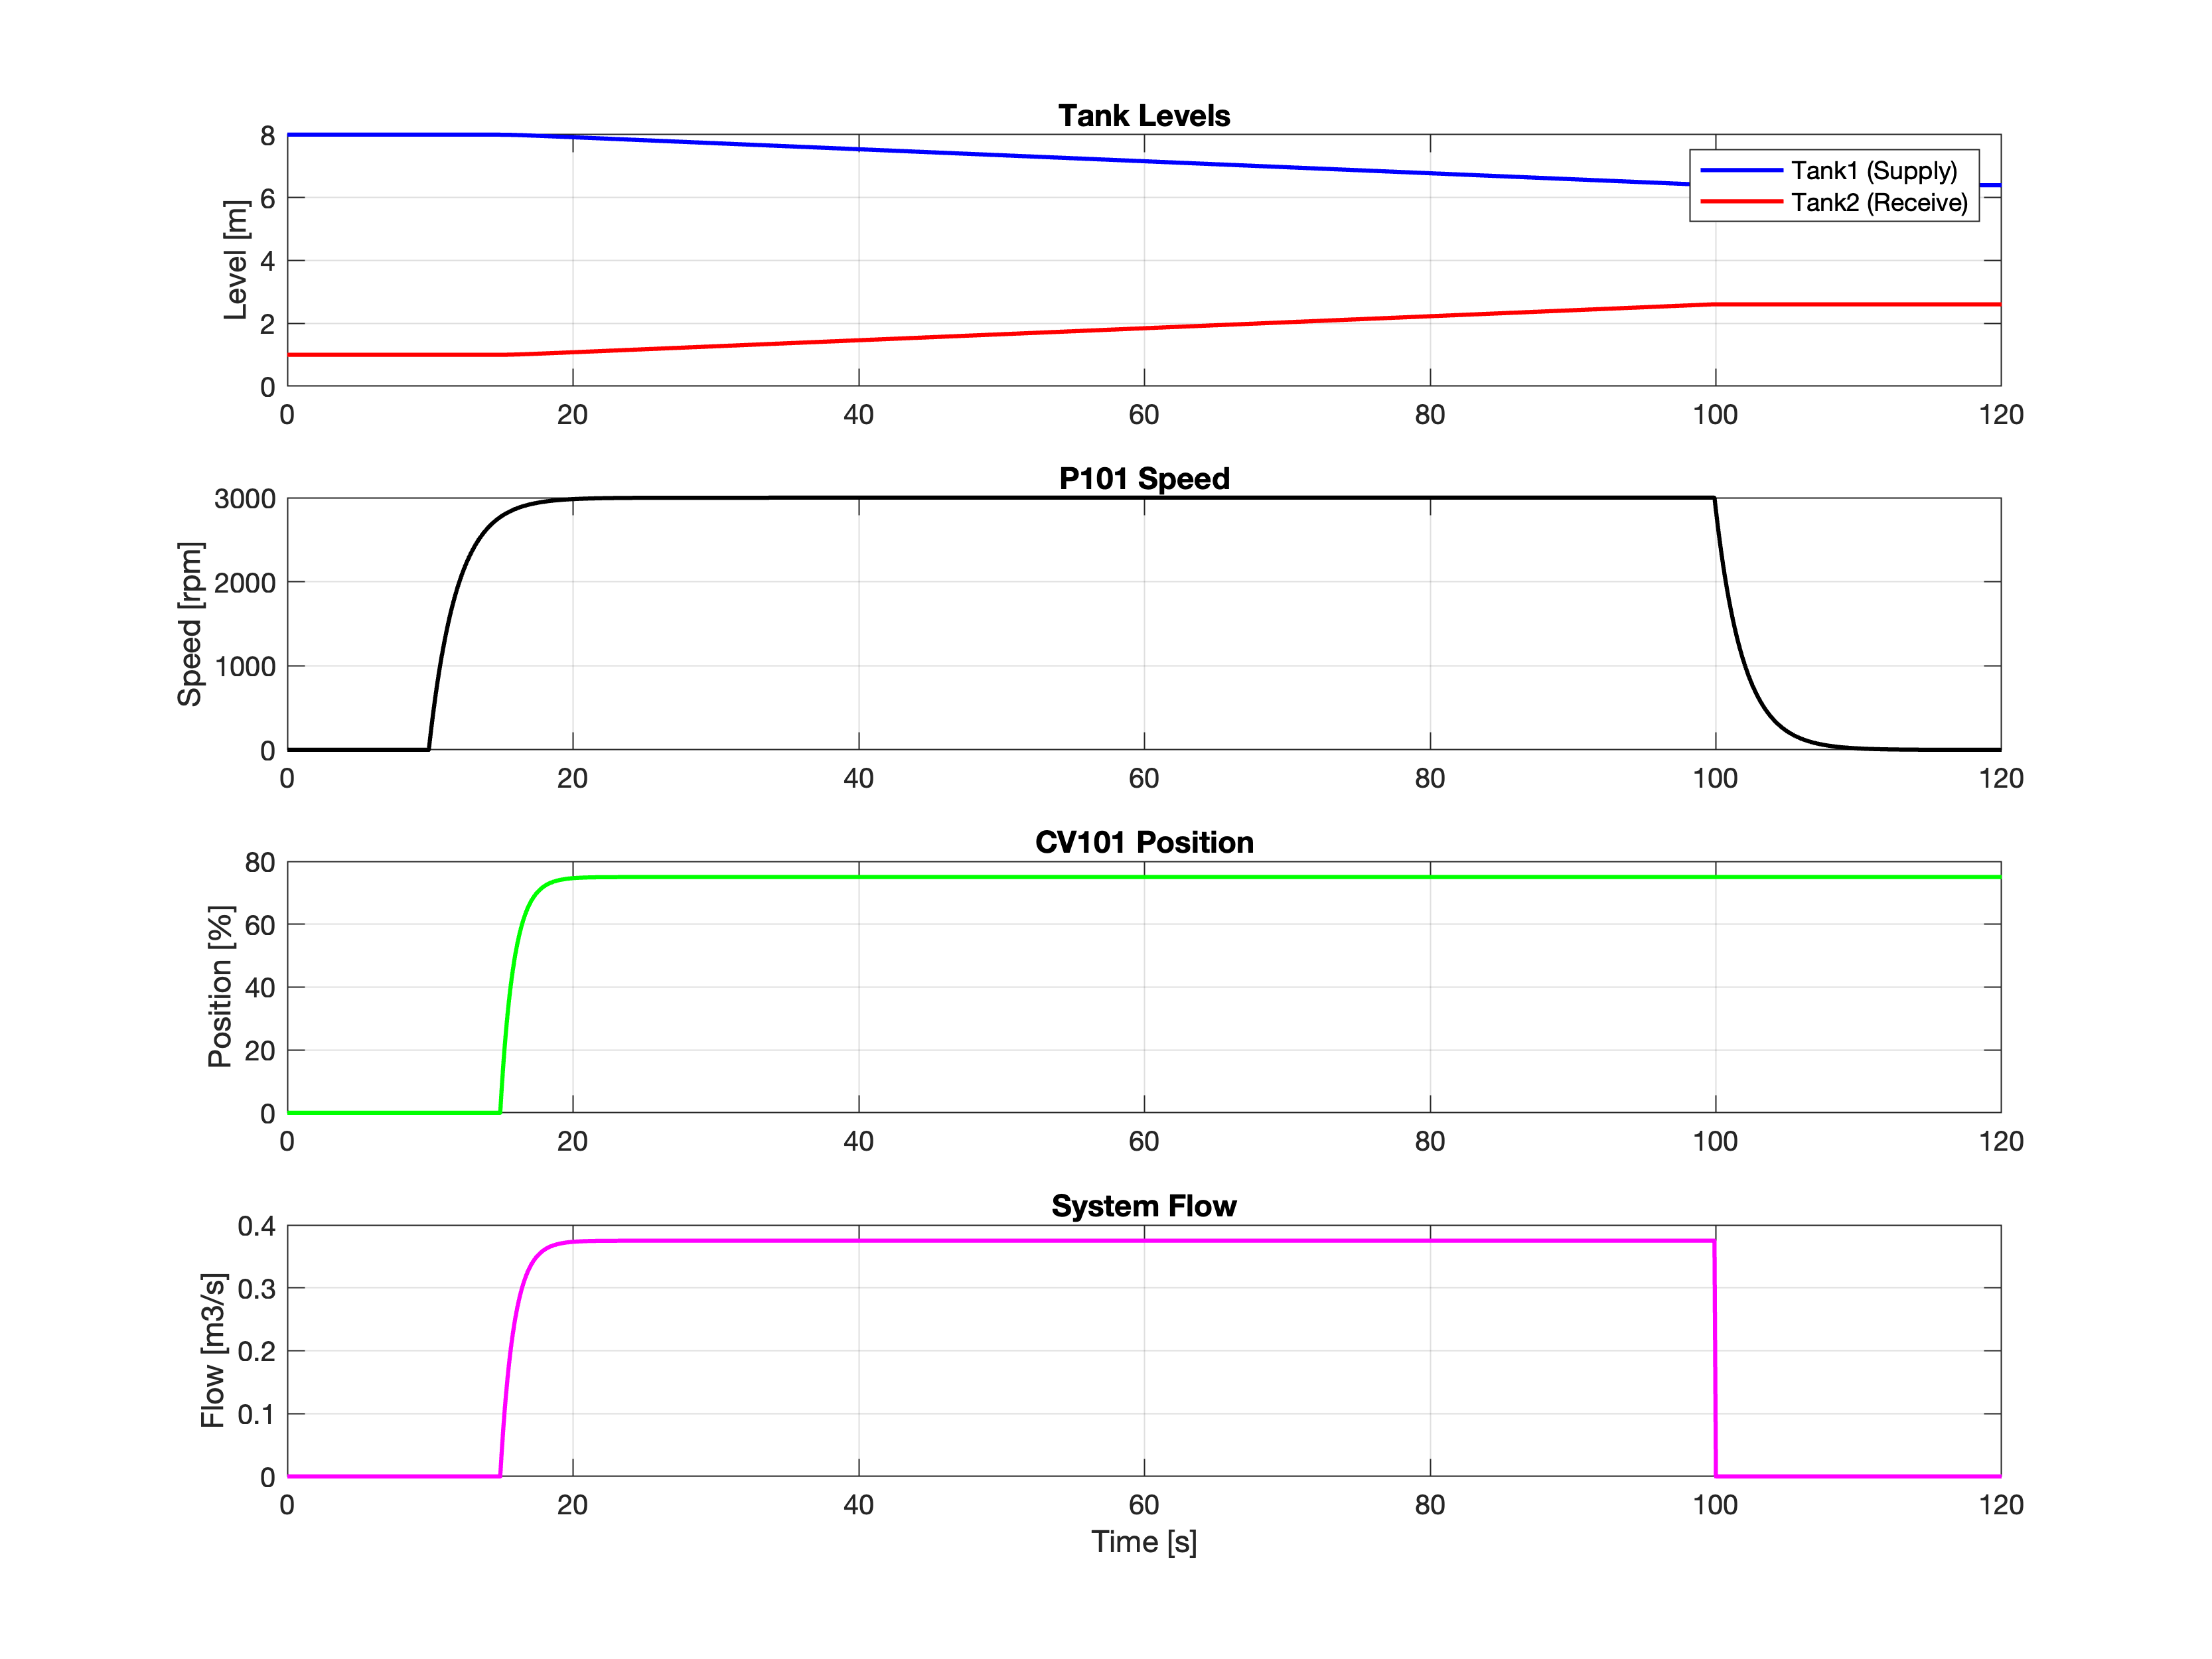
\includegraphics[width=0.9\textwidth]{images/pump_tank.png}
    \caption{Pump, Tank, and Valve integration example.}
    \label{fig:pump_tank}
\end{figure}

\section{\texttt{HistorianExample.m}}
A backend-focused benchmark script. It evaluates the performance of the \texttt{ETagDatabase} mapping system and ensures that the \texttt{EHistorian} can log thousands of data points without memory fragmentation, outputting a clean MATLAB timetable.

\begin{figure}[H]
    \centering
    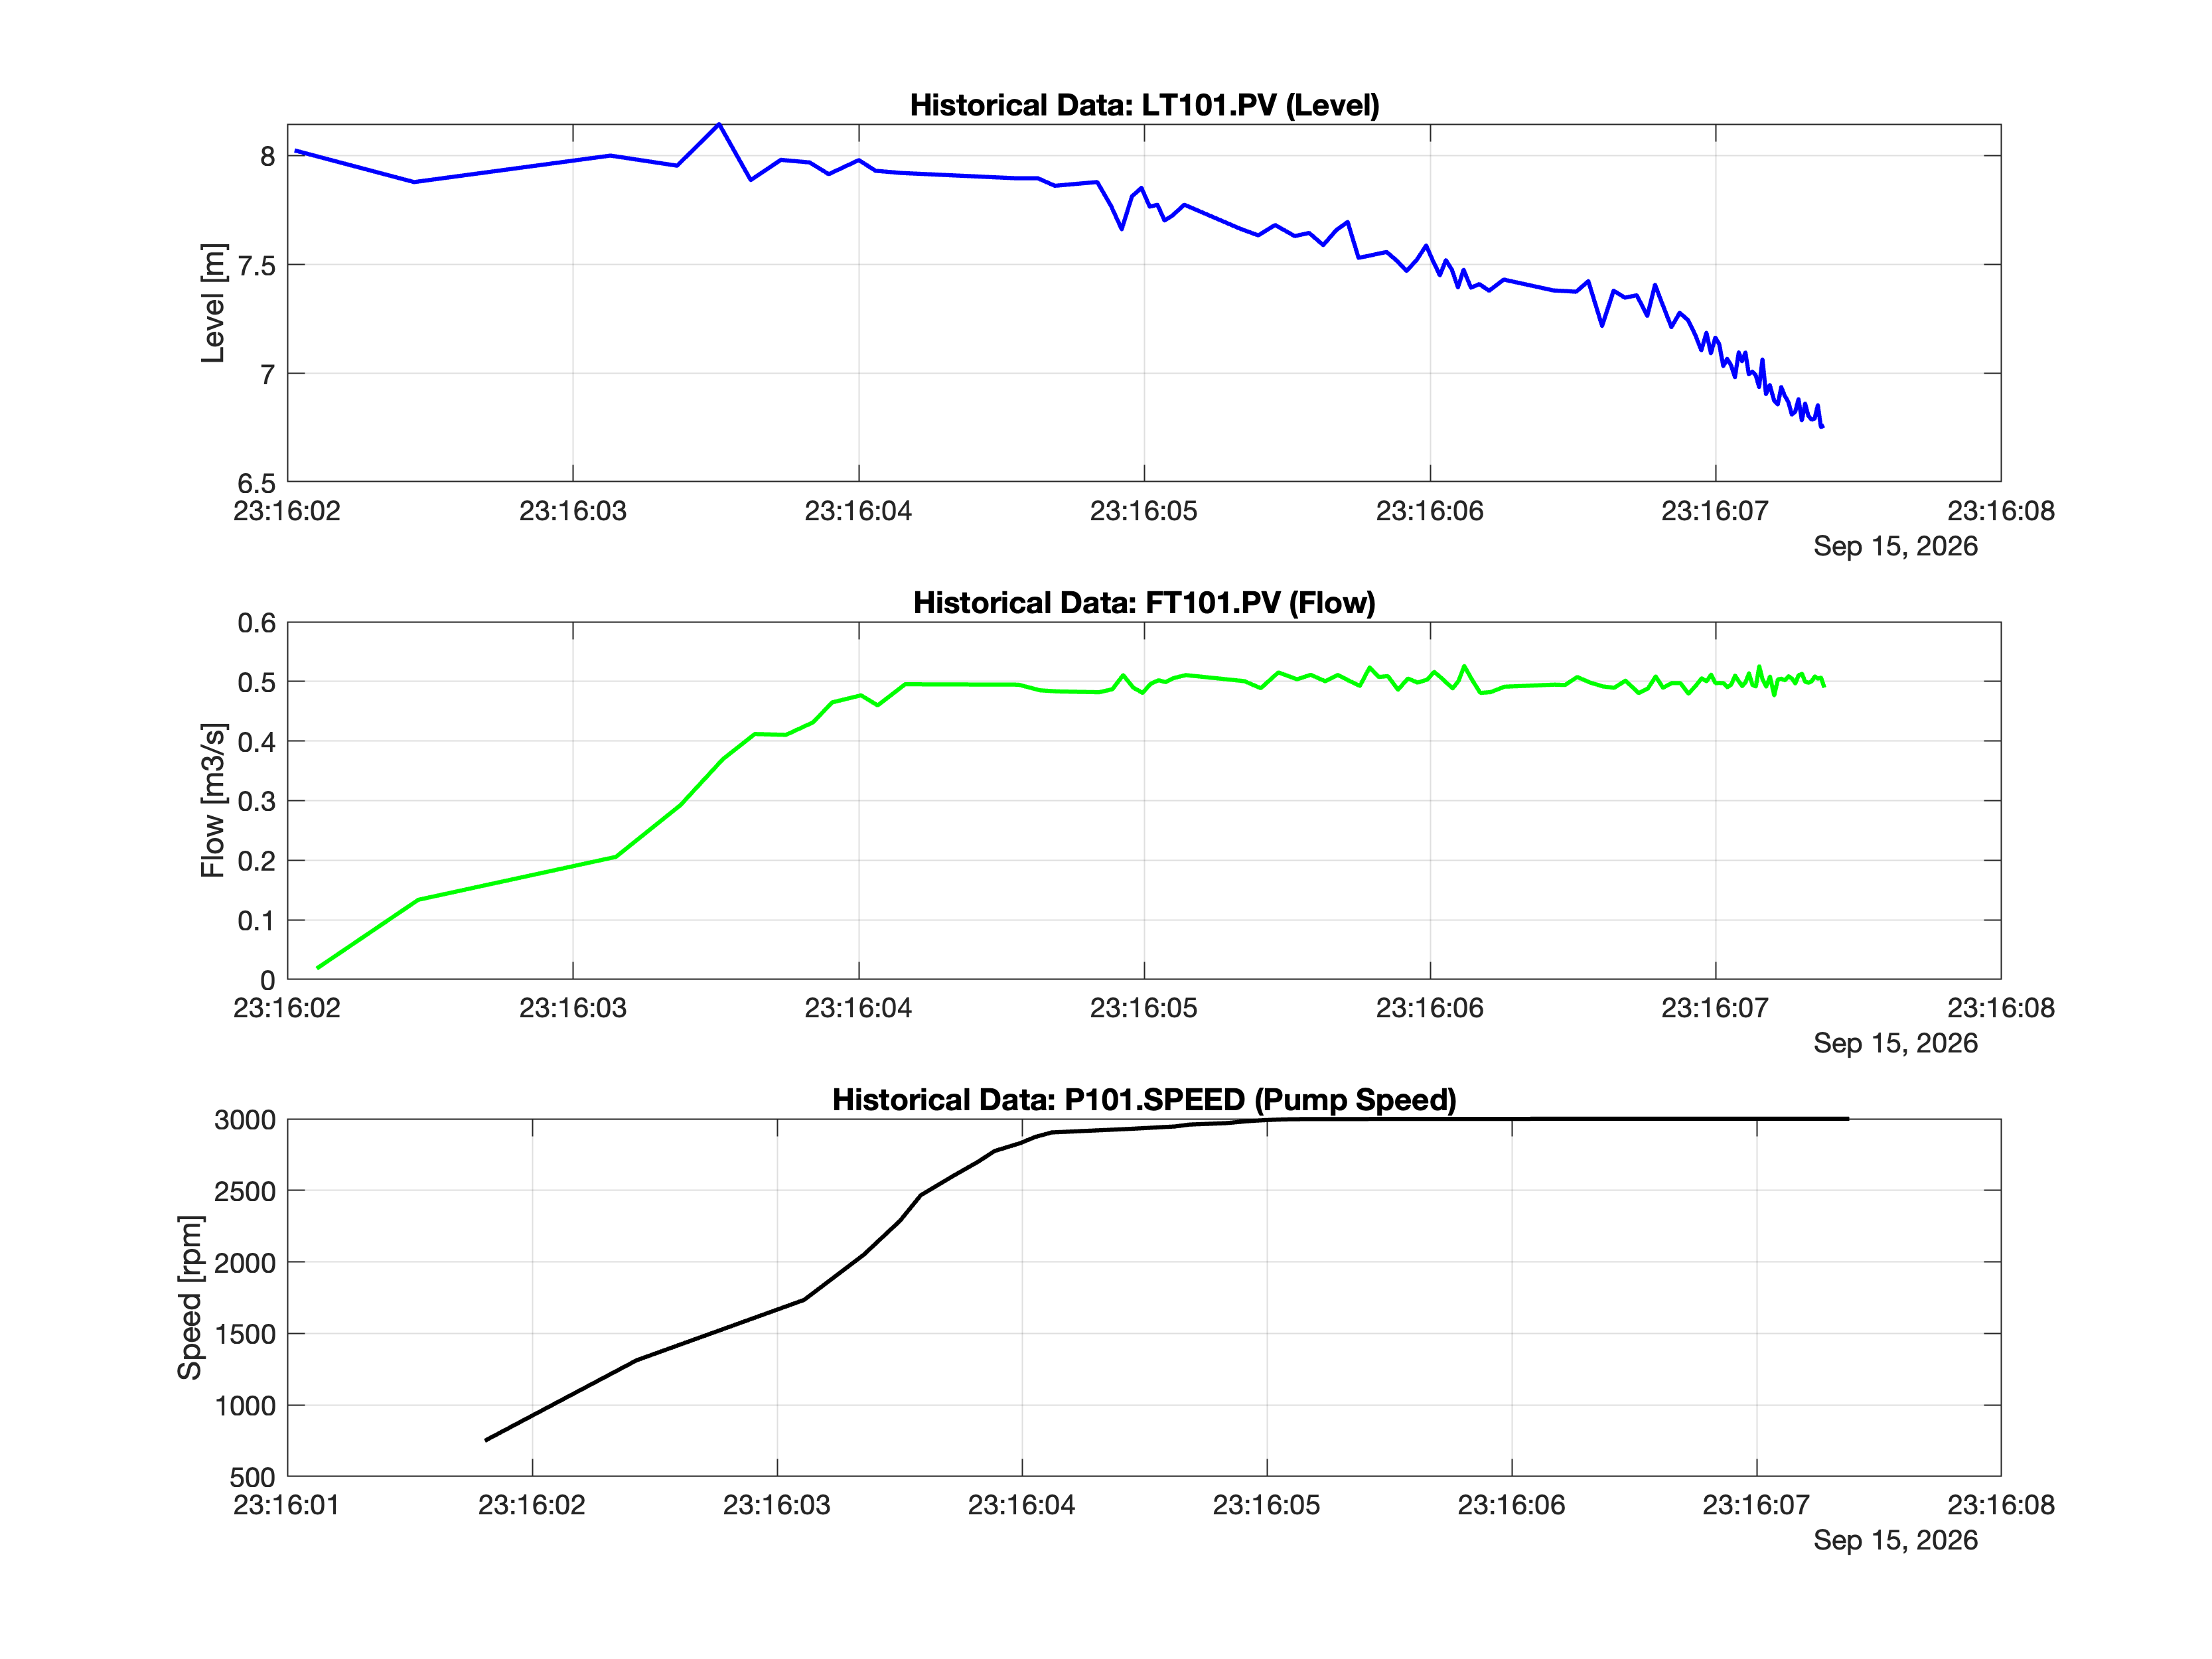
\includegraphics[width=0.9\textwidth]{images/historian.png}
    \caption{Historian time-series generation and native MATLAB plotting.}
    \label{fig:historian_example}
\end{figure}

\section{\texttt{InstrumentationExample.m} (Mid Phase)}
Highlights the sensory degradation layer. It runs a side-by-side comparison of the actual physics engine state versus the noisy, 4-20mA clamped signal output by the \texttt{ETransmitter}, including a mid-simulation cable break fault.

\begin{figure}[H]
    \centering
    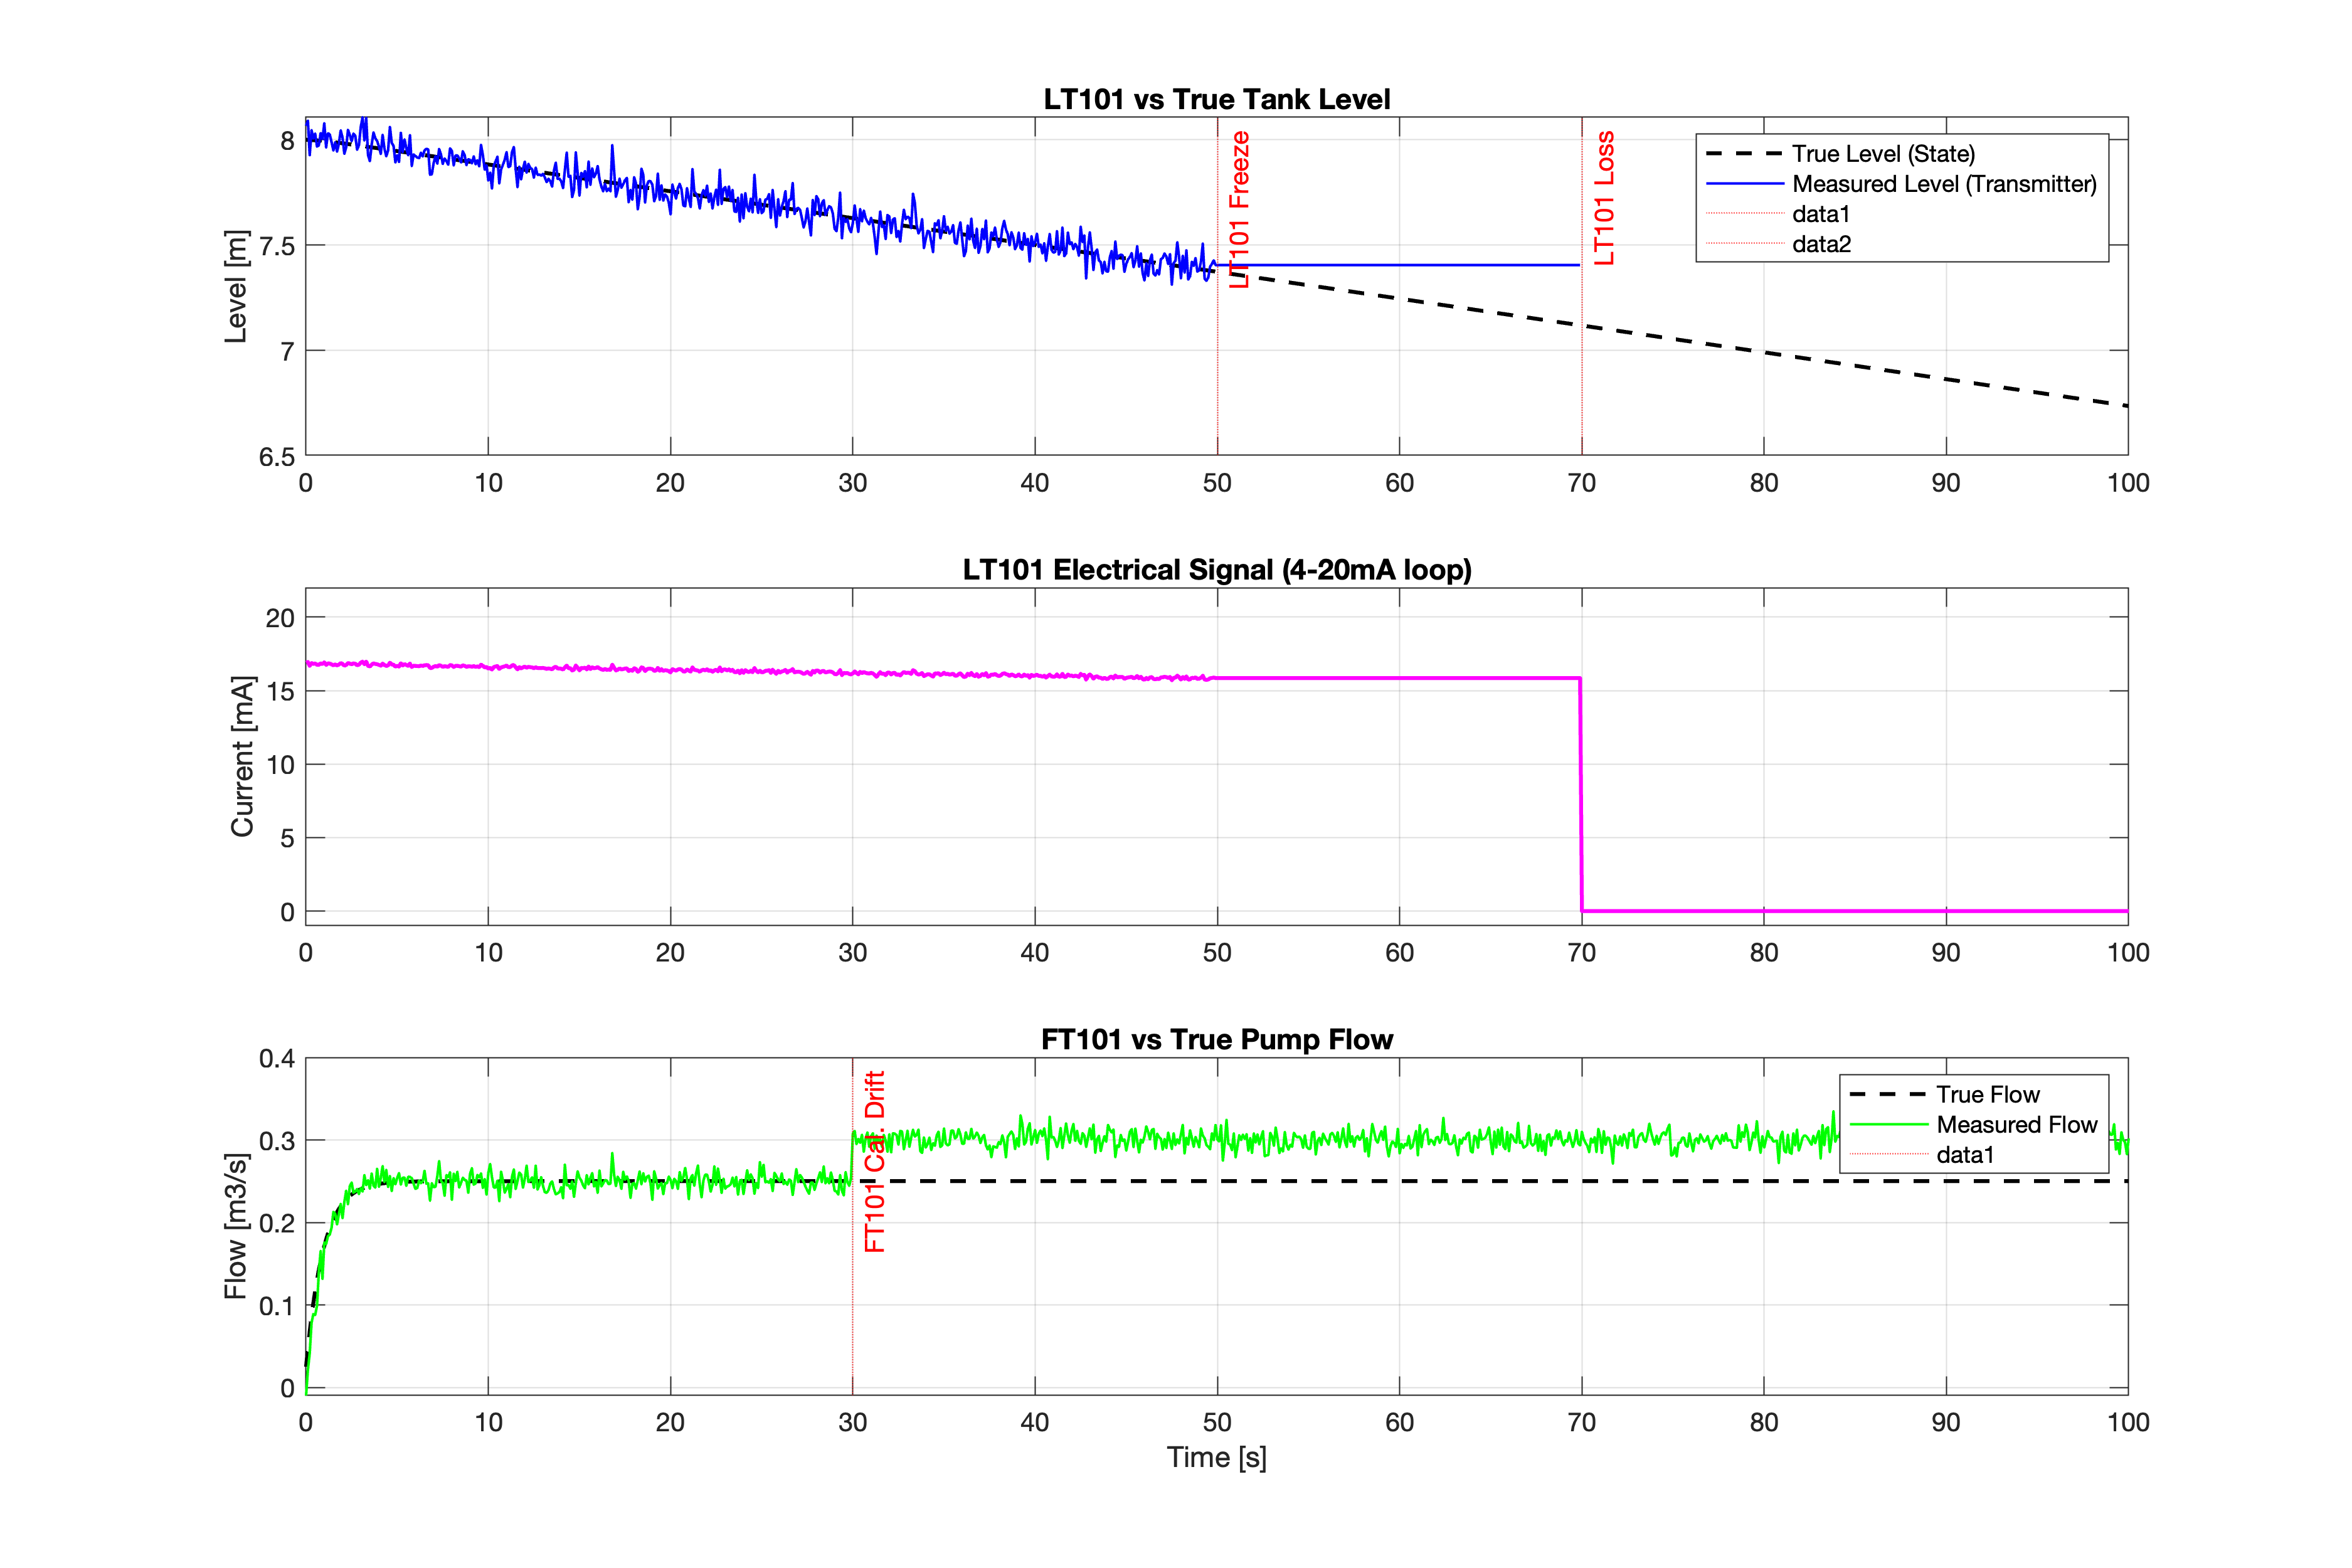
\includegraphics[width=0.9\textwidth]{images/instrumentation.png}
    \caption{Instrumentation Example showing Ground Truth vs. Measured signals with Noise and Faults.}
    \label{fig:instrumentation}
\end{figure}

\section{\texttt{FullFactoryExample.m} (Final Phase)}
The culmination of the project. It builds an entire plant:
\begin{itemize}
    \item Two source tanks pumped by VFD-controlled motors through control valves.
    \item A Mixer combining the two flows with different concentrations.
    \item A Heater applying thermal energy.
    \item A Filter accumulating pressure drop.
    \item A final product tank.
\end{itemize}
The script injects a \textit{Heater Element Failure} and a \textit{Filter Rupture} dynamically. It uses the \texttt{ESimulationEngine} to run the plant and extracts data natively from the \texttt{EHistorian} for final visualization.

\begin{figure}[H]
    \centering
    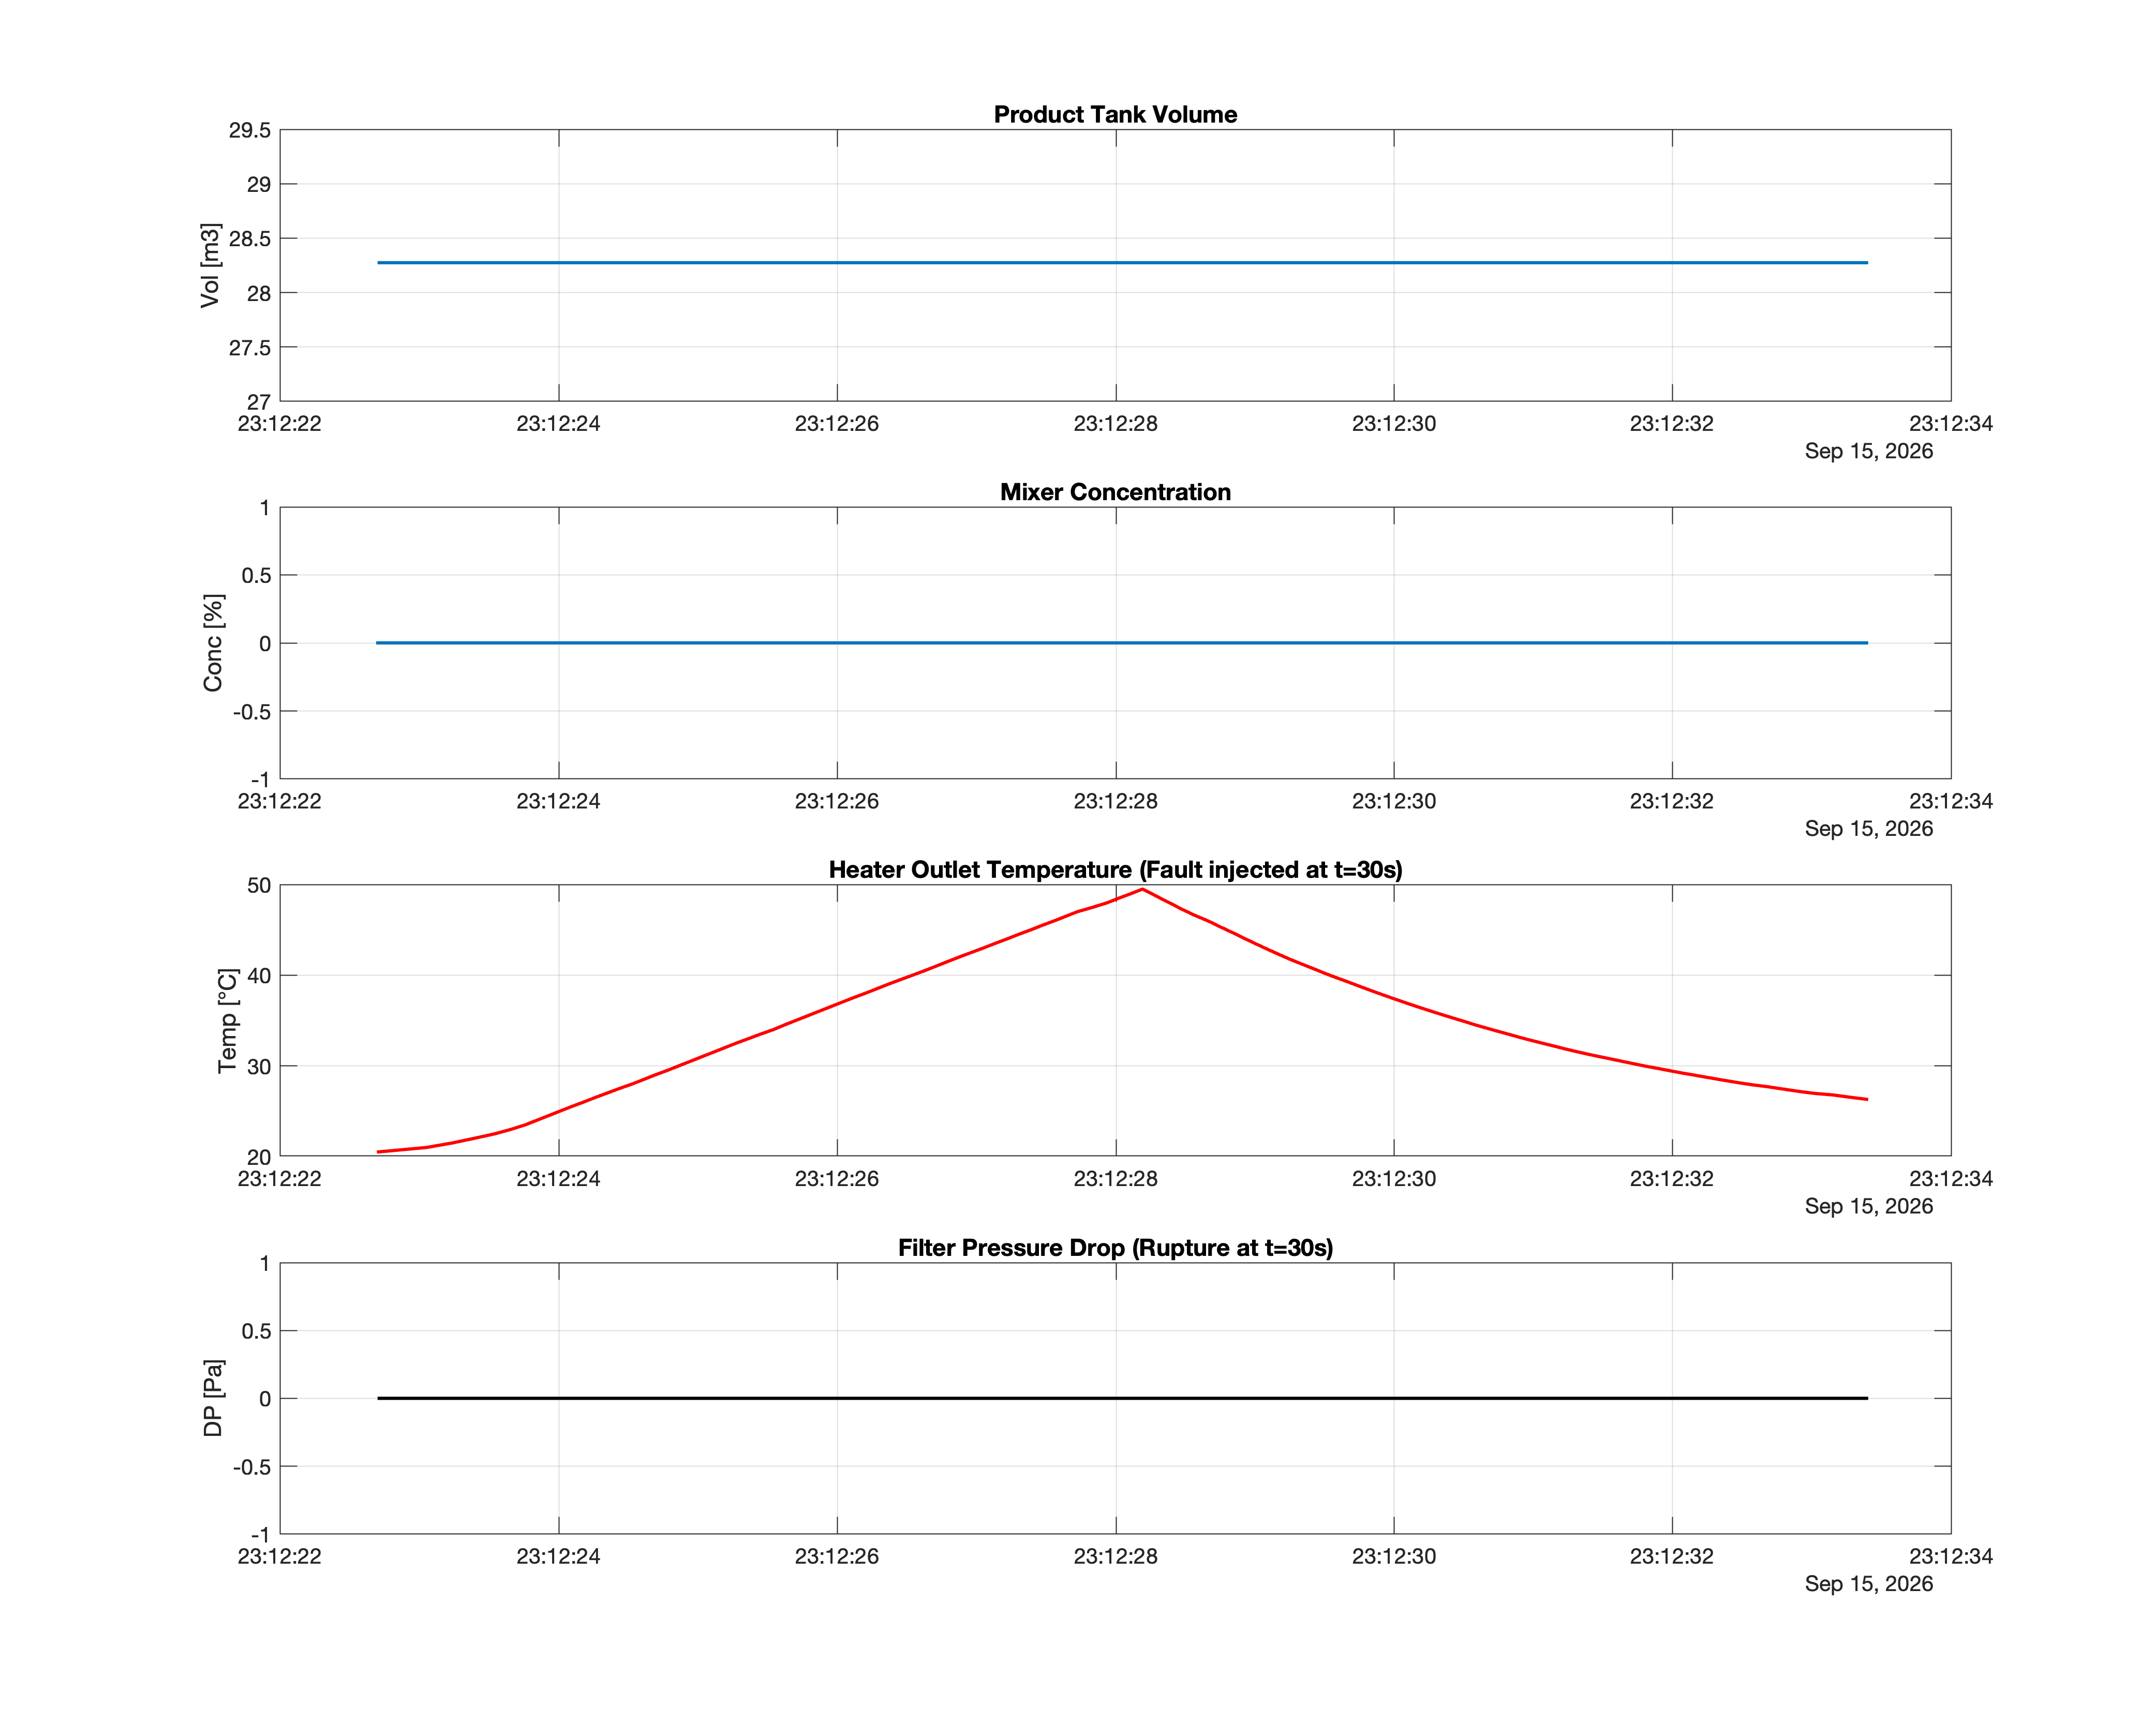
\includegraphics[width=0.9\textwidth]{images/full_factory.png}
    \caption{Full Factory Simulation showcasing Historian Tag extraction for Volume, Concentration, Temperature, and Pressure Drop over time.}
    \label{fig:full_factory}
\end{figure}

\chapter{User Manual: How to Build Your Own Plant}

\section{Step 1: Instantiating the Environment}
To begin, you must create the \texttt{EFactory} which automatically provisions the Tag Database and Historian.
\begin{lstlisting}
factory = EFactory();
\end{lstlisting}

\section{Step 2: Declaring Equipment}
Create physical process units using their constructors. You can override default parameters such as dimensions or rated limits.
\begin{lstlisting}
% Create a 10m high tank
TankA = ETank("ID", "TK101", "Diameter", 5, "Height", 10, "InitialLevel", 8);

% Create a motor and its VFD
MotorA = EMotor("ID", "MTR101", "RatedSpeed", 1500, "RatedPower", 15);
VFD_A = EVFD("ID", "VFD101", "Motor", MotorA);
\end{lstlisting}

\section{Step 3: Attaching Instrumentation}
To read variables into the SCADA system, attach Transmitters to the process equipment.
\begin{lstlisting}
% Monitor TankA's level with a maximum range of 10m
LT_A = ELevelTransmitter("ID", "LT101", "Target", TankA, "RangeMax", 10);
\end{lstlisting}

\section{Step 4: Registration}
Add all instantiated components to the factory. This step ensures that the Tag Database registers them for polling.
\begin{lstlisting}
factory.add(TankA);
factory.add(MotorA);
factory.add(VFD_A);
factory.add(LT_A);
\end{lstlisting}

\section{Step 5: Running the Simulation}
Initialize the \texttt{ESimulationEngine} with the factory and a discrete time step (e.g., $dt = 0.5$ seconds). In a custom loop, you can script hydraulic connections (mapping flows between tanks and pumps), inject faults, and call \texttt{factory.update(dt)}.
\begin{lstlisting}
engine = ESimulationEngine(factory, 0.5);
for k = 1:100
    % Inject a fault at step 50
    if k == 50
        LT_A.injectFault('SignalLoss');
    end
    
    % Step the physics and log tags
    factory.update(0.5);
end
\end{lstlisting}

\section{Step 6: Extracting Data}
Once the loop finishes, extract the generated timetables natively.
\begin{lstlisting}
% Extract native MATLAB timetable
ttLevel = factory.Historian.getHistory("LT101.PV");

% Plot time-series data natively
plot(ttLevel.Time, ttLevel.Value);
\end{lstlisting}

\chapter{Conclusion}
To summarize, this project demonstrates the feasibility of combining rigorous mathematical physics with modern object-oriented software design in MATLAB. Rather than relying on simple scripts, the Digital Twin architecture acts as a comprehensive sandbox. It enables engineers to test complex control loops, validate SCADA alarming strategies, and generate high-fidelity datasets for Machine Learning applications, all before any physical hardware is deployed.

\end{document}
